% Report of results from Ramsay simulation experiment
% David Lawrence Miller
% d.l.miller@bath.ac.uk

% Started : 8th April 2009

\documentclass[a4paper,10pt]{amsart}

% Load some packages
\usepackage{times, amsmath, amssymb, amsfonts, url, natbib, bm, rotating,multirow,graphicx}

% top matter
\title{Smoothing over irregular shapes using the Schwarz-Christoffel transform}
\author{David Lawrence Miller}
\email{d.l.miller@bath.ac.uk}
\address{Mathematical Sciences, University of Bath, Bath, United Kingdom}

% Shortcuts
% Probability
\newcommand{\prob}[1]{\mathbb{P}\left[ #1 \right]}
% Hovitz-Thompson
\newcommand{\HT}{\hat{\tau}_{HT}}
% Schwarz-Christoffel
\newcommand{\sch}{Schwarz-Christoffel }
% fprime
\newcommand{\fprime}{f^\prime(z)}
% figure reference command
\newcommand{\fig}[1]{\emph{fig.} (\ref{#1})}
% figure reference command (start of sentance
\newcommand{\Fig}[1]{\emph{Fig.} (\ref{#1})}
% equation reference command
\newcommand{\eqn}[1]{\emph{eqn.} (\ref{#1})}
% phi inverse
\newcommand{\phiinv}{\phi^{-1}}
% use other phi
\newcommand{\ophi}{\phi}
\renewcommand{\phi}{\varphi}




\begin{document}

% The abstract
\begin{abstract}
Following on from looking at the Ramsay horseshoe, other polygon mappings are simulated from and transformed with the \sch transform.
\end{abstract}


% New theorem for theorems
\newtheorem{thm}{Theorem}[section]

%New theorem for definitions
\newtheorem{defn}{Definition}[section]

\maketitle



\section{Looking at other domains}

Why? Say something about breaking things.


\section{Figure 9}

We first take a look at the polygon shown in \fig{fig9} and map to both the rectangle and the unit disk. Data was then generated from two multivariate Normal distributions. Taking this as truth, samples were taken and a smooth fit using thin plate regression spllines using \texttt{mgcv}.


\begin{figure}
\centering
% trim order l b r t
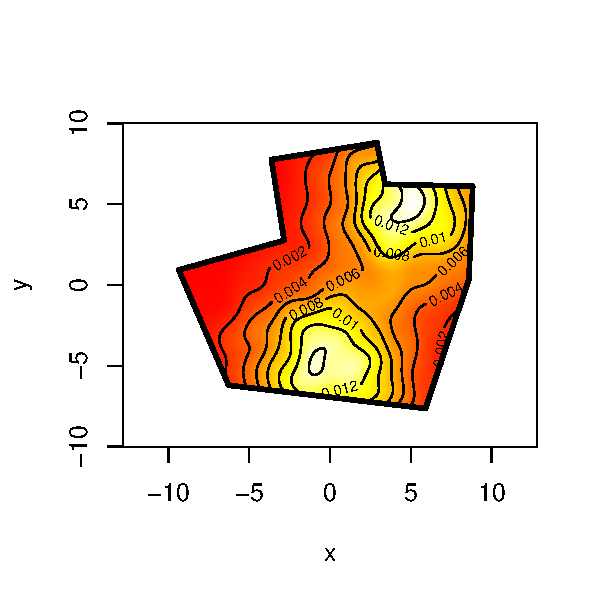
\includegraphics{figs-otherdomains/fig9.pdf} \\
\caption{The heatmap of the polygon's generated density.}
\label{fig9}
% generated by /phd-smoothing/sc-writeup/figs-otherdomains/fig9.R
\end{figure}




Using rectangle and disk mapping. How was the density simulated. Why doesn't it work as well as tprs.



\section{Wigglytop}


Blahblah blah what is it etc

In our initial simulations, we picked 10,000 from 250,000 points generated over the shape. We then added Normal noise ($\sigma^2=0.02$.) In this domain it would seem that picking the vertices to amap to the corners of the rectangle is crucial.

In the first attempt the SC Toolbox was allowed to pick the corners automatically using the \texttt{crrectmap} routine, this routine also uses the CRDT algorithm to increase the numerical stability of the solution. \Fig{wigglyfirstcomp} shows the comparison between the truth, the \sch transform with thin plate regression splines and using thin plate regression splines without the transform. The MSE was calculated for both models and there was not a large difference between the two. The thin plate method reported an MSE of 9.221594e-05 while using the transform reported 9.154827e-05. Although the difference is very small, it is obvious from looking at the heatmaps that something has gone wrong.

\begin{figure}
\centering
% trim order l b r t
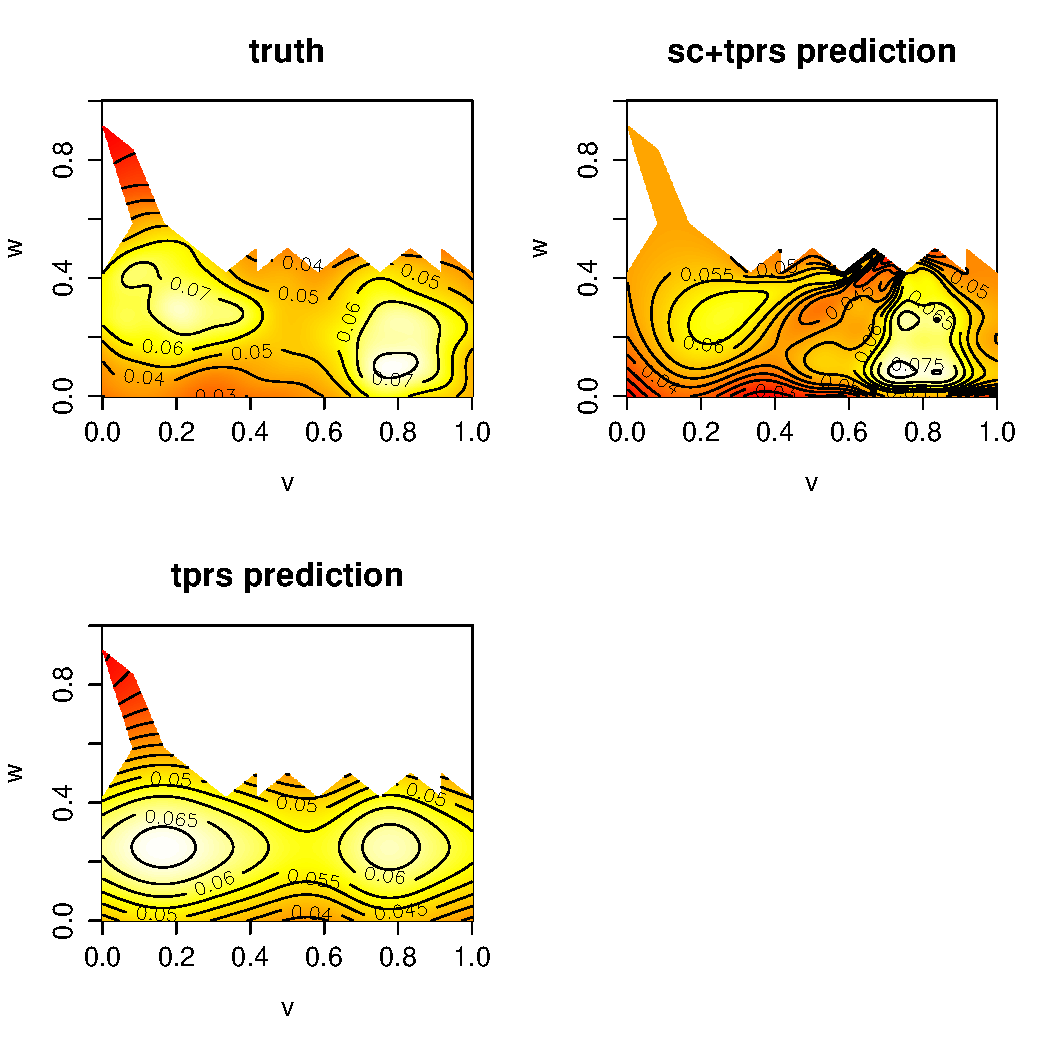
\includegraphics[width=3in]{figs-otherdomains/wigglytop-first.pdf} \\
\caption{Clockwise from top left: truth, the fit from the transformation method and the fit from a standard thin plate regression spline. The transform is when \texttt{crrectmap} is allowed to choose the vertices to map to the corners of the rectangle.}
\label{wigglyfirstcomp}
% generated by /phd-smoothing/wigglytop/fit...
\end{figure}

To investigate this, the vertices that are to be mapped to the corners were selected manually, still using \texttt{crrectmap}. 

sc+tprs 6.043222e-05 
tprs 9.157006e-05 


\begin{figure}
\centering
% trim order l b r t
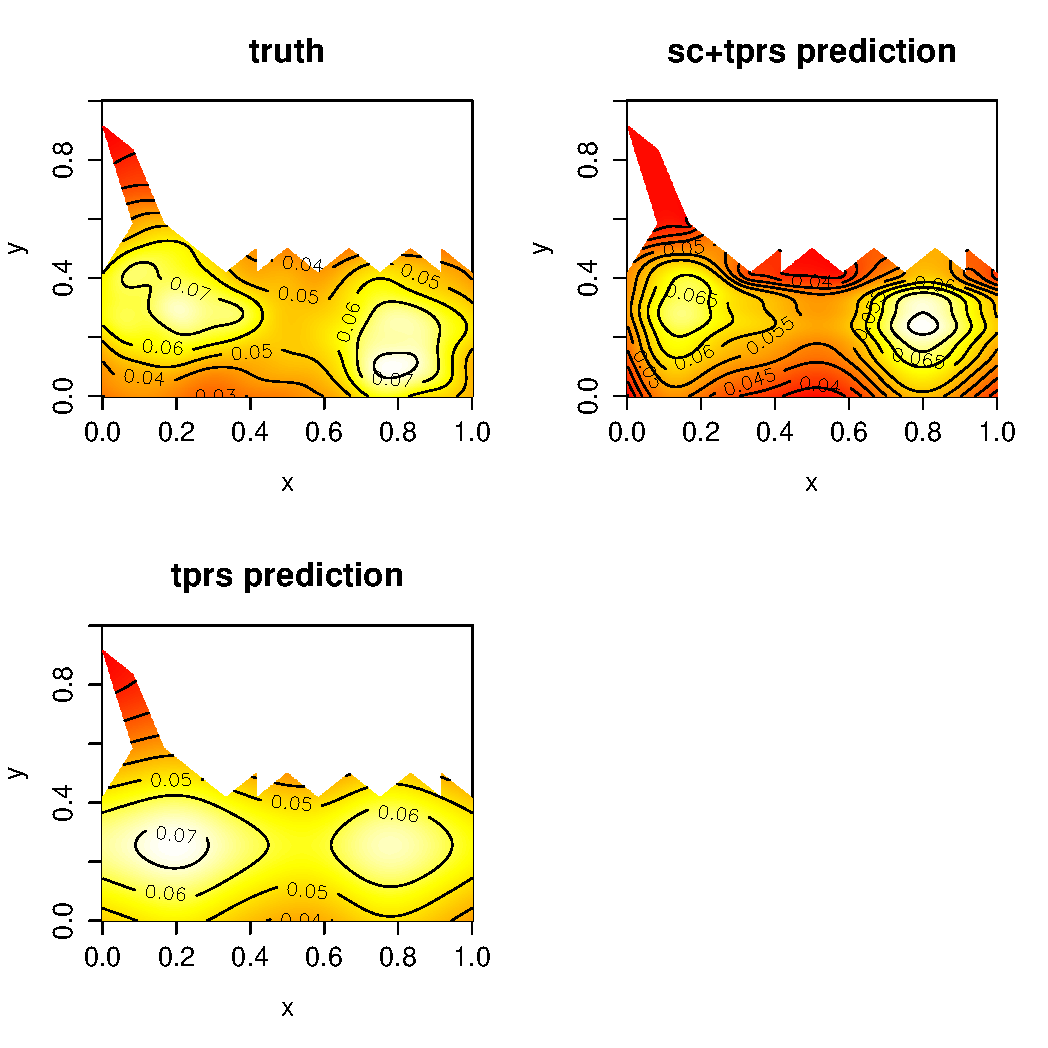
\includegraphics[width=3in]{figs-otherdomains/wigglytop-second.pdf} \\
\caption{Clockwise from top left: truth, the fit from the transformation method and the fit from a standard thin plate regression spline. The transform is when vertices to map to corners are specified manually.}
\label{wigglyseccomp}
% generated by /phd-smoothing/wigglytop/fit...
\end{figure}




this is just using rectmap
Second try, as before but with the real corners selected
sc+tprs 7.358453e-05 
tprs 9.51009e-05 










\bibliographystyle{plainnat}
\bibliography{sc-refs}



\end{document}
